\section{ROS 2 Humble Foundations}

\begin{frame}{From Python to ROS 2}
\framesubtitle{Python provides logic; ROS 2 connects that logic to the robotic system}
\begin{center}
\large
\textbf{A drone is not one program. It is a team of communicating components.}
\end{center}
\pause
\begin{columns}[T,onlytextwidth]
\begin{column}{0.30\textwidth}
\begin{block}{Perception}
Camera acquisition and object detection.
\end{block}
\end{column}
\hfill
\begin{column}{0.30\textwidth}
\begin{block}{Mission Logic}
Trajectory generation and inspection decisions.
\end{block}
\end{column}
\hfill
\begin{column}{0.30\textwidth}
\begin{block}{Flight Interface}
Telemetry reception and PX4 setpoint publication.
\end{block}
\end{column}
\end{columns}
\begin{exampleblock}{ROS 2 Role}
ROS 2 provides the communication and integration framework that allows these components to discover one another and exchange typed information.
\end{exampleblock}
\end{frame}




\begin{frame}{What Is ROS 2?}
\framesubtitle{A modular software framework for building robot systems}
\begin{block}{Intuitive Definition}
ROS 2 is a collection of software libraries, command-line tools, conventions, and communication mechanisms used to create and integrate robotic applications.
\end{block}
\pause
\begin{exampleblock}{Team Analogy}
Imagine a technical team in which each specialist has one responsibility. ROS 2 provides the shared language, communication channels, addresses, and rules that let the specialists cooperate.
\end{exampleblock}
\begin{alertblock}{Important Distinction}
ROS 2 is not the computer's operating system. Ubuntu manages hardware, files, memory, users, and processes. ROS 2 runs on top of Ubuntu and organizes communication between robotics software components.
\end{alertblock}
\end{frame}

% \begin{frame}{Why Use ROS 2 in Robotics?}
% \framesubtitle{Complex systems become understandable when responsibilities are separated}
% \footnotesize
% \begin{itemize}
% \item \textbf{Modularity:} camera, mission, control, and logging components can be developed separately.
% \item \textbf{Typed communication:} interfaces define the structure of exchanged data.
% \item \textbf{Observability:} terminal tools expose nodes, topics, services, actions, and parameters.
% \item \textbf{Language flexibility:} components may be implemented in Python or C++.
% \item \textbf{Reuse:} packages and standard interfaces reduce duplicated engineering work.
% \item \textbf{Distributed operation:} communicating components may run in different processes or on different computers.
% \end{itemize}
% \begin{exampleblock}{Drone Project Connection}
% ROS 2 connects mission logic, PX4 interfaces, camera bridges, perception programs, visualization, and evidence collection without forcing them into one monolithic program.
% \end{exampleblock}
% \end{frame}




\begin{frame}{Why Use ROS 2?}
\framesubtitle{ROS 2 helps separate programs work together}

\footnotesize

\begin{center}
    \textbf{A complete robot is not one large program.}\\[0.2em]
    It is a team of smaller programs with different responsibilities.
\end{center}

\pause

\begin{columns}[T,onlytextwidth]
    \begin{column}{0.30\textwidth}
        \begin{block}{Separate}
            Each component performs one clear task:
            camera, mission, control, perception, or logging.
        \end{block}
    \end{column}
    \hfill
    \begin{column}{0.30\textwidth}
        \begin{block}{Connect}
            ROS 2 allows the components to exchange structured messages
            through defined interfaces.
        \end{block}
    \end{column}
    \hfill
    \begin{column}{0.30\textwidth}
        \begin{block}{Observe}
            ROS 2 tools help engineers inspect which components are
            running and what information they exchange.
        \end{block}
    \end{column}
\end{columns}

\pause

\begin{exampleblock}{Drone Project Example}
    The camera produces images
    \(\rightarrow\)
    the detector identifies objects
    \(\rightarrow\)
    the mission node uses the observations
    \(\rightarrow\)
    the results are visualized and recorded.
\end{exampleblock}

\begin{alertblock}{Central Idea}
    ROS 2 does not fly the drone and does not detect objects.
    It is the communication and integration framework that helps
    the specialized software components work together.
\end{alertblock}

\end{frame}


\begin{frame}{Course Compatibility Contract}
\framesubtitle{Every command and exercise targets one supported baseline}
\begin{center}
\Large\textbf{Ubuntu 22.04 LTS + ROS 2 Humble Hawksbill}
\end{center}
\begin{block}{Student Rule}
Use the versions specified by the internship repository. Do not silently replace Humble commands or packages with instructions written for another ROS 2 distribution.
\end{block}
\begin{alertblock}{Why This Matters}
Package names, supported platforms, simulator combinations, APIs, and setup instructions may differ between ROS 2 distributions. Newer does not automatically mean compatible with this project.
\end{alertblock}
\end{frame}

\subsection{Environment and First Observation}

\begin{frame}[fragile]{Live Check 1: Load ROS 2 Humble}
\framesubtitle{Each new terminal must receive the ROS 2 environment}
\begin{block}{Execute}
\begin{verbatim}
source /opt/ros/humble/setup.bash
printenv ROS_DISTRO
which ros2
ros2 --help
\end{verbatim}
\end{block}
\begin{exampleblock}{Expected Evidence}
\texttt{ROS\_DISTRO} should report \texttt{humble}, and \texttt{which ros2} should locate the ROS 2 command-line executable.
\end{exampleblock}
\begin{alertblock}{Interpretation}
\texttt{source} changes the current shell environment. It does not reinstall ROS 2. Repeat it in every new terminal unless the project defines an approved automatic setup.
\end{alertblock}
\end{frame}

\begin{frame}[fragile]{Live Check 2: Diagnose the Environment}
\framesubtitle{Verify the installation before blaming application code}
\begin{block}{Execute}
\begin{verbatim}
ros2 doctor --report
\end{verbatim}
\end{block}
\begin{exampleblock}{What to Inspect}
Confirm the ROS 2 distribution, platform, middleware information, network interfaces, and package environment. Read warnings in context rather than treating every line as a fatal error.
\end{exampleblock}
\begin{alertblock}{Engineering Habit}
Preserve the command and complete output when asking for help. A screenshot of only the last line may hide the actual cause.
\end{alertblock}
\end{frame}

\begin{frame}[fragile]{Live Demonstration: Start Turtlesim}
\framesubtitle{Use a small system before connecting the drone stack}
\begin{columns}[T,onlytextwidth]
\begin{column}{0.48\textwidth}
\begin{block}{Terminal 1}
\begin{verbatim}
source /opt/ros/humble/setup.bash
ros2 run turtlesim turtlesim_node
\end{verbatim}
\end{block}
\end{column}
\begin{column}{0.48\textwidth}
\begin{block}{Terminal 2}
\begin{verbatim}
source /opt/ros/humble/setup.bash
ros2 run turtlesim turtle_teleop_key
\end{verbatim}
\end{block}
\end{column}
\end{columns}
\begin{exampleblock}{What to Observe}
Two executables run as separate processes. One displays the simulated turtle; the other converts keyboard input into movement commands.
\end{exampleblock}
\begin{alertblock}{Terminal Focus}
Keep Terminal 2 active while pressing arrow keys. Stop each foreground process deliberately with \texttt{Ctrl+C}.
\end{alertblock}
\end{frame}

\subsection{The ROS 2 Graph and Nodes}

\begin{frame}{The ROS 2 Graph}
\framesubtitle{A live map of components and communication relationships}
\begin{center}
Nodes $+$ topics $+$ services $+$ actions $+$ parameters $=$ \textbf{ROS 2 graph}
\end{center}
\begin{block}{Intuition}
The graph is not a file stored once. It is the changing network of ROS 2 entities that currently exist and communicate while the system runs.
\end{block}
\begin{exampleblock}{Drone Example}
An orbit controller, PX4 bridge, image bridge, detector, and evidence logger appear as nodes connected through named interfaces.
\end{exampleblock}
\end{frame}





\begin{frame}{A Simple ROS 2 Computation Graph}
\framesubtitle{How a mobile robot exchanges sensor data and motion commands}

\footnotesize

\begin{center}
    \textbf{Obstacle Detector}
    \(\xleftarrow{\quad \texttt{/scan} \quad}\)
    \textbf{Robot Driver}
    \(\xleftarrow{\quad \texttt{/cmd\_vel} \quad}\)
    \textbf{Motion Controller}
\end{center}

\vspace{0.15cm}

\begin{columns}[T,onlytextwidth]

    \begin{column}{0.48\textwidth}
        \begin{block}{Sensor Information}
            The robot driver acts as a
            \textbf{publisher} on:

            \begin{center}
                \texttt{/scan}
            \end{center}

            It publishes laser measurements using:

            \begin{center}
                \texttt{sensor\_msgs/msg/LaserScan}
            \end{center}

            Any node interested in obstacle detection can
            \textbf{subscribe} to this topic.
        \end{block}
    \end{column}

    \hfill

    \begin{column}{0.48\textwidth}
        \begin{exampleblock}{Motion Commands}
            The robot driver acts as a
            \textbf{subscriber} on:

            \begin{center}
                \texttt{/cmd\_vel}
            \end{center}

            It receives velocity commands using:

            \begin{center}
                \texttt{geometry\_msgs/msg/Twist}
            \end{center}

            A controller publishes the desired linear and
            angular velocities on this topic.
        \end{exampleblock}
    \end{column}

\end{columns}

\pause

\begin{alertblock}{Key Intuition}
    The robot driver connects ROS 2 to the robot or simulator.
    It publishes what the robot senses and subscribes to what
    the software wants the robot to do.
\end{alertblock}

\end{frame}



\begin{frame}{ROS 2 Names and Namespaces}
\framesubtitle{Organizing communication in single-robot and multi-robot systems}

\footnotesize

\begin{block}{Names Work Like Filesystem Paths}
    ROS 2 resources use structured names beginning with
    \texttt{/}. A namespace adds a common prefix that groups
    related nodes and topics.
\end{block}

\begin{center}
\renewcommand{\arraystretch}{1.25}
\begin{tabular}{c@{\hspace{0.5cm}}c}
    \textbf{Single Robot}
    &
    \textbf{Two Robots}
    \\[0.1cm]

    \texttt{/cmd\_vel}
    &
    \texttt{/drone\_1/cmd\_vel}
    \\

    \texttt{/scan}
    &
    \texttt{/drone\_1/scan}
    \\[0.1cm]

    &
    \texttt{/drone\_2/cmd\_vel}
    \\

    &
    \texttt{/drone\_2/scan}
\end{tabular}
\end{center}

\pause

\begin{exampleblock}{Why Namespaces Matter}
    Both robots may use the same node design and message types,
    while their namespaces keep their commands and sensor data
    separate.
\end{exampleblock}

\begin{alertblock}{Drone Project Connection}
    A command published to \texttt{/drone\_1/cmd\_vel} should not
    accidentally control \texttt{drone\_2}.
\end{alertblock}

\end{frame}


\begin{frame}{The ROS 2 Graph}
    \centering
    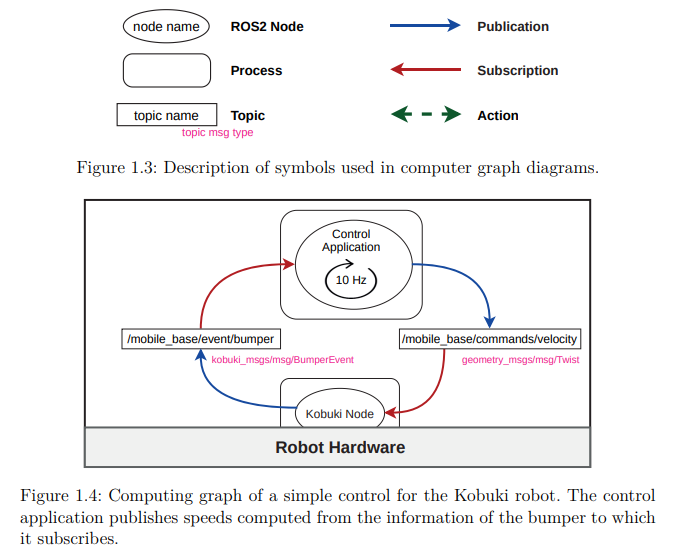
\includegraphics[width=0.6\textwidth]{./images/computation_graph.png}\cite{martin-rico-ros2}
\end{frame}

\begin{frame}{What Is a ROS 2 Node?}
\framesubtitle{One software specialist responsible for one part of the robot}

\footnotesize

\begin{center}
    \textbf{A robotic system is a team of specialized programs.}\\[0.2em]
    In ROS 2, each running specialist is called a \textbf{node}.
\end{center}

\pause

\begin{columns}[T,onlytextwidth]
    \begin{column}{0.30\textwidth}
        \begin{block}{Receive}
            A node can receive information from other nodes.

            \vspace{0.1cm}
            \textbf{Example:} receive a camera image.
        \end{block}
    \end{column}
    \hfill
    \begin{column}{0.30\textwidth}
        \begin{block}{Process}
            A node performs one focused software task.

            \vspace{0.1cm}
            \textbf{Example:} detect an object.
        \end{block}
    \end{column}
    \hfill
    \begin{column}{0.30\textwidth}
        \begin{block}{Send}
            A node can share its result with other nodes.

            \vspace{0.1cm}
            \textbf{Example:} publish detections.
        \end{block}
    \end{column}
\end{columns}

\pause

\begin{exampleblock}{Drone Project Example}
    The \textbf{camera node} publishes images
    \(\rightarrow\)
    the \textbf{detector node} identifies objects
    \(\rightarrow\)
    the \textbf{mission node} uses the observations
    \(\rightarrow\)
    the \textbf{logger node} records evidence.
\end{exampleblock}

\begin{alertblock}{Central Idea}
    A node is not a physical sensor or part of the drone.
    It is a running software component with one clear responsibility
    inside the complete robotic system.
\end{alertblock}

\end{frame}

\begin{frame}{ROS 2 Demonstration}
    \centering
    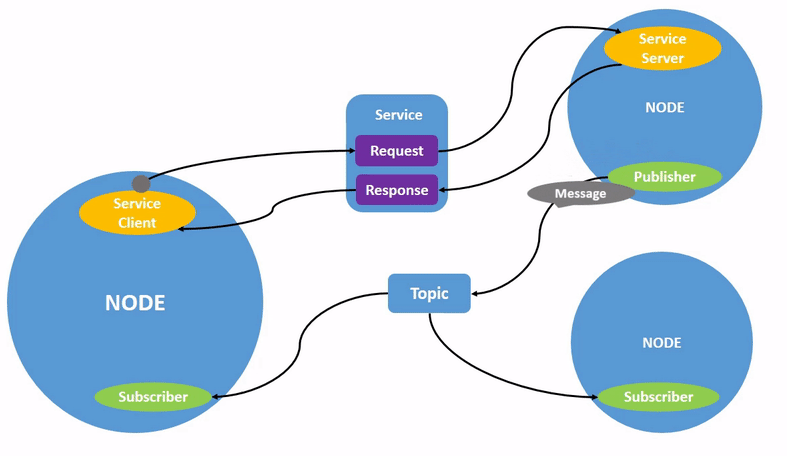
\includegraphics[width=0.8\textwidth]{./images/NodesTopicandService1.png}
\end{frame}

\begin{frame}{ROS 2 Demonstration}
    \centering
    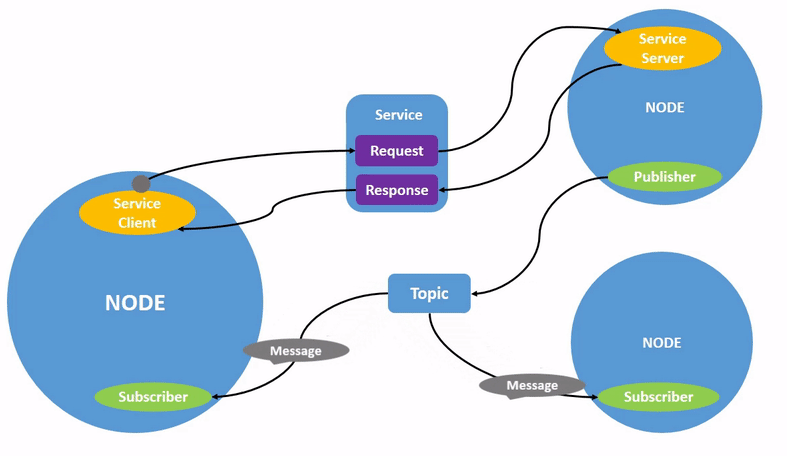
\includegraphics[width=0.8\textwidth]{./images/NodesTopicandService2.png}
\end{frame}


\begin{frame}[fragile]{Live Tutorial: Discover Nodes}
\framesubtitle{Ask the running system who is participating}
\begin{block}{Keep Turtlesim Running, Then Execute}
\begin{verbatim}
ros2 node list
ros2 node info /turtlesim
ros2 node info /teleop_turtle
\end{verbatim}
\end{block}
\begin{exampleblock}{Read the Output}
\texttt{ros2 node list} identifies active node names. \texttt{ros2 node info} reveals publishers, subscribers, services, actions, and interfaces associated with one node.
\end{exampleblock}
\begin{alertblock}{Project Transfer}
Later, use \texttt{ros2 node list} to verify that the orbit controller, bridges, and perception nodes actually started. A terminal window alone is not sufficient evidence.
\end{alertblock}
\end{frame}


\begin{frame}{Reading \texttt{ros2 node info} }
\framesubtitle{Do not read every line first; identify the node's communication roles}

\footnotesize

\begin{block}{The Main Question}
    What information does the \texttt{/turtlesim} node
    \textbf{receive}, \textbf{produce}, and \textbf{provide on request}?
\end{block}

\pause

\begin{columns}[T,onlytextwidth]

    \begin{column}{0.31\textwidth}
        \begin{exampleblock}{Receives}
            \centering
            \textbf{Subscribers}

            \vspace{0.12cm}

            \texttt{/turtle1/cmd\_vel}

            \vspace{0.12cm}

            \scriptsize
            The node receives movement commands as
            \texttt{Twist} messages.
        \end{exampleblock}
    \end{column}

    \hfill

    \begin{column}{0.31\textwidth}
        \begin{exampleblock}{Produces}
            \centering
            \textbf{Publishers}

            \vspace{0.12cm}

            \texttt{/turtle1/pose}

            \texttt{/turtle1/color\_sensor}

            \vspace{0.12cm}

            \scriptsize
            The node publishes its position and sensor information.
        \end{exampleblock}
    \end{column}

    \hfill

    \begin{column}{0.31\textwidth}
        \begin{exampleblock}{Provides}
            \centering
            \textbf{Services and Actions}

            \vspace{0.12cm}

            \texttt{/spawn}

            \texttt{/reset}

            \texttt{/rotate\_absolute}

            \vspace{0.12cm}

            \scriptsize
            Other nodes can request operations or send a goal.
        \end{exampleblock}
    \end{column}

\end{columns}

\pause

\begin{center}
    \textbf{\color{um6p-dark}
    Receive commands
    \(\longrightarrow\)
    update the simulation
    \(\longrightarrow\)
    publish observations}
\end{center}

\begin{alertblock}{Do Not Be Overwhelmed}
    Entries containing \texttt{parameter} and \texttt{/rosout} are normal
    ROS~2 support interfaces. At the beginning, focus only on the interfaces
    directly related to the turtle's motion and observations.
\end{alertblock}

\end{frame}


\subsection{Topics, Publishers, Subscribers, and Messages}

\begin{frame}{Topics: Continuous Information Channels}
\framesubtitle{Publishers send data; subscribers receive matching data}
\begin{center}
\textbf{Publisher} $\longrightarrow$ named topic $\longrightarrow$ \textbf{Subscriber}
\end{center}
\begin{block}{Intuition}
A topic resembles a radio channel. Publishers transmit without addressing one specific receiver. Any compatible subscriber may listen to the named channel.
\end{block}
\begin{exampleblock}{Drone Examples}
Camera images, vehicle odometry, desired paths, detection results, and telemetry are natural topic data because they may be produced repeatedly over time.
\end{exampleblock}
\end{frame}

\begin{frame}{Publishers and Subscribers}
\framesubtitle{Communication roles are independent from node names}
\begin{columns}[T,onlytextwidth]
\begin{column}{0.47\textwidth}
\begin{block}{Publisher}
Creates messages of a defined type and sends them on a named topic.
\end{block}
\end{column}
\hfill
\begin{column}{0.47\textwidth}
\begin{block}{Subscriber}
Registers interest in a named topic and executes a callback when compatible data arrives.
\end{block}
\end{column}
\end{columns}
\begin{exampleblock}{Many-to-Many Possibility}
One publisher may serve several subscribers, and several publishers may write compatible messages to the same topic. System design must make this intentional.
\end{exampleblock}
\end{frame}

\begin{frame}{Messages: Typed Data Contracts}
\framesubtitle{Every topic carries a defined data structure}
\begin{block}{Intuition}
A message type is a standardized form. It defines the fields and field types that communicating components agree to exchange.
\end{block}
\begin{exampleblock}{Examples}
A velocity command may contain linear and angular components. An image message includes pixel data and metadata. PX4 odometry includes estimated position, velocity, orientation, and timestamps.
\end{exampleblock}
\begin{alertblock}{Why Types Matter}
A subscriber cannot safely interpret arbitrary bytes. Both sides must agree on the interface, units, coordinate conventions, and semantic meaning.
\end{alertblock}
\end{frame}

\begin{frame}[fragile]{Live Tutorial: Inspect Topics}
\framesubtitle{Discover names, types, rates, and current data}
\scriptsize
\begin{verbatim}
ros2 topic list
ros2 topic list -t
ros2 topic info /turtle1/cmd_vel --verbose
ros2 topic type /turtle1/cmd_vel
ros2 interface show geometry_msgs/msg/Twist
ros2 topic echo /turtle1/pose
ros2 topic hz /turtle1/pose
\end{verbatim}
\begin{block}{Observation Sequence}
Find the topic, identify its type, inspect the interface fields, observe actual messages, and measure publication frequency.
\end{block}
\begin{alertblock}{Stop Streaming Commands}
\texttt{ros2 topic echo} and \texttt{ros2 topic hz} continue until interrupted. Stop them with \texttt{Ctrl+C}.
\end{alertblock}
\end{frame}


\begin{frame}[fragile]{Discover the Available Topics}
\framesubtitle{Which communication channels currently exist?}

\footnotesize

\begin{block}{List the Active Topics}
\begin{verbatim}
ros2 topic list
\end{verbatim}
\end{block}

% \begin{exampleblock}{Observed Output}
% \begin{verbatim}
% /parameter_events
% /rosout
% /turtle1/cmd_vel
% /turtle1/color_sensor
% /turtle1/pose
% \end{verbatim}
% \end{exampleblock}

\begin{block}{Intuitive Interpretation}
Each topic is a named communication channel:

\begin{itemize}
    \setlength{\itemsep}{0.16em}
    \item \texttt{/turtle1/cmd\_vel}: receives motion commands;
    \item \texttt{/turtle1/pose}: publishes the turtle state;
    \item \texttt{/turtle1/color\_sensor}: publishes sensed background color.
\end{itemize}
\end{block}

\begin{alertblock}{Central Idea}
\texttt{ros2 topic list} shows which communication channels exist,
but it does not show their message types or current data.
\end{alertblock}

\end{frame}

% -----------------------------------------------------------------------------
\begin{frame}[fragile]{Discover Topics and Their Types}
\framesubtitle{What kind of message travels through each channel?}

\footnotesize

\begin{block}{Execute}
\begin{verbatim}
ros2 topic list -t
\end{verbatim}
\end{block}

% \begin{exampleblock}{Observed Output}
% \begin{verbatim}
% /parameter_events [rcl_interfaces/msg/ParameterEvent]
% /rosout [rcl_interfaces/msg/Log]
% /turtle1/cmd_vel [geometry_msgs/msg/Twist]
% /turtle1/color_sensor [turtlesim/msg/Color]
% /turtle1/pose [turtlesim/msg/Pose]
% \end{verbatim}
% \end{exampleblock}

\begin{block}{How to Read One Line}
\begin{center}
\texttt{/turtle1/cmd\_vel}
\quad
\(\longrightarrow\)
\quad
\texttt{geometry\_msgs/msg/Twist}
\end{center}

The first element is the \textbf{topic name}.  
The value in brackets is the \textbf{message type}.
\end{block}

\begin{alertblock}{Central Idea}
A topic is the channel. The message type defines the structure of the
information allowed to travel through that channel.
\end{alertblock}

\end{frame}

% -----------------------------------------------------------------------------
\begin{frame}[fragile]{Inspect One Topic}
\framesubtitle{Who is connected to the velocity-command channel?}

\footnotesize

\begin{columns}[T,onlytextwidth]

    % --- LEFT COLUMN: The Terminal Action ---
    \begin{column}{0.48\textwidth}
        \begin{block}{1. Execute the Command}
\begin{verbatim}
ros2 topic info /turtle1/cmd_vel --verbose
\end{verbatim}
        \end{block}

        \begin{exampleblock}{2. The Terminal Output}
\begin{verbatim}
Type: geometry_msgs/msg/Twist

Publisher count: 0
Subscription count: 1
...
\end{verbatim}
        \end{exampleblock}
    \end{column}

    % --- RIGHT COLUMN: The Engineering Meaning ---
    \begin{column}{0.48\textwidth}
        \begin{block}{3. Intuitive Interpretation}
            Let's break down exactly what the system is telling us:
            \begin{itemize}
                \setlength{\itemsep}{0.3em}
                \item \textbf{Type:} The expected message structure is \texttt{Twist} (linear \& angular velocity).
                \item \textbf{Sub count = 1:} One node (\texttt{turtlesim}) is actively listening and waiting for commands.
                \item \textbf{Pub count = 0:} Absolutely no node is currently sending commands into this topic.
            \end{itemize}
        \end{block}
    \end{column}

\end{columns}

        \vspace{0.1cm}

        \begin{alertblock}{4. The Engineering Conclusion}
            The turtle is fully awake and ready to receive velocity commands, but no controller program is currently publishing them. \textbf{This explains exactly why the turtle is stationary on your screen.}
        \end{alertblock}
\end{frame}

% -----------------------------------------------------------------------------
\begin{frame}[fragile]{Inspect the Message Contract}
\framesubtitle{What exact information must a velocity command contain?}

\footnotesize

\begin{columns}[T,onlytextwidth]

    % --- LEFT COLUMN: The Terminal Commands ---
    \begin{column}{0.48\textwidth}
        \begin{block}{1. Find the Message Type}
\begin{verbatim}
$ ros2 topic type /turtle1/cmd_vel
geometry_msgs/msg/Twist
\end{verbatim}
        \end{block}
    \end{column}

    % --- RIGHT COLUMN: The Engineering Translation ---
    \begin{column}{0.48\textwidth}
        \pause
        \begin{block}{3. The Engineering Contract}
            A \texttt{Twist} message is the universal ROS 2 standard for rigid body movement. It enforces two 3D vectors:
            \begin{itemize}
                \setlength{\itemsep}{0.3em}
                \item \textbf{\texttt{linear}:} Translational velocity (meters/second).
                \item \textbf{\texttt{angular}:} Rotational velocity (radians/second).
            \end{itemize}
        \end{block}

        \vspace{0.15cm}
    \end{column}

\end{columns}

        \begin{alertblock}{4. Application to the Turtle (and Drone)}
            Because the turtle lives in a flat 2D world, it only needs two of these six variables:
            \begin{itemize}
                \setlength{\itemsep}{0.2em}
                \item \texttt{linear.x} to drive forward/backward.
                \item \texttt{angular.z} to spin left/right.
            \end{itemize}
            \vspace{0.1cm}
            % \textit{Note: Later in the internship, your 3D drone will use all 6 variables to fly!}
        \end{alertblock}
\end{frame}
% -----------------------------------------------------------------------------
\begin{frame}[fragile]{Observe Live Topic Data}
\framesubtitle{What is the turtle publishing right now?}

\footnotesize

\begin{columns}[T,onlytextwidth]

    % --- LEFT COLUMN: The Terminal Action ---
    \begin{column}{0.48\textwidth}
        \begin{block}{1. Execute the Echo Command}
            \textit{Listen to the live stream of data:}
\begin{verbatim}
$ ros2 topic echo /turtle1/pose
\end{verbatim}
        \end{block}

        \begin{exampleblock}{2. The Continuous Output}
\begin{verbatim}
x: 5.544445 y: 5.544445
theta: 0.0  linear_velocity: 0.0
angular_velocity: 0.0
\end{verbatim}
        \end{exampleblock}
    \end{column}

    % --- RIGHT COLUMN: The Engineering Analysis ---
    \begin{column}{0.48\textwidth}
        \begin{block}{3. Breaking Down the Telemetry}
            \begin{itemize}
                \setlength{\itemsep}{0.25em}
                \item \textbf{\texttt{x} and \texttt{y}:} Current 2D position in the grid.
                \item \textbf{\texttt{theta}:} Current orientation (yaw).
                \item \textbf{\texttt{velocities}:} Current physical speed.
                \item \textbf{\texttt{---}:} Separates messages. Because this data publishes continuously (e.g., at 62 Hz), the terminal will stream endlessly until you press \texttt{Ctrl+C}.
            \end{itemize}
        \end{block}
    \end{column}

\end{columns}

        \begin{alertblock}{4. The Drone Connection}
            Right now, both velocities are zero (the turtle is stationary). \textbf{Later this week, you will use this exact same command to read the live GPS and IMU data streaming from your 3D drone in Gazebo!}
        \end{alertblock}
\end{frame}

% -----------------------------------------------------------------------------
\begin{frame}[fragile]{Measure the Publication Frequency}
\framesubtitle{How frequently does the pose topic deliver new messages?}

\footnotesize

\begin{columns}[T,onlytextwidth]

    % --- LEFT COLUMN: The Terminal Action ---
    \begin{column}{0.48\textwidth}
        \begin{block}{1. Execute the Hertz Command}
            \textit{Measure the data rate in real-time:}
\begin{verbatim}
$ ros2 topic hz /turtle1/pose
\end{verbatim}
        \end{block}

        \begin{exampleblock}{2. The Terminal Output}
\begin{verbatim}
average rate: 62.504
  min: 0.015s
  max: 0.017s
  std dev: 0.00047s
  window: 64
\end{verbatim}
        \end{exampleblock}
    \end{column}

    % --- RIGHT COLUMN: The Engineering Math ---
    \begin{column}{0.48\textwidth}
        \begin{block}{3. The Math \& Interpretation}
            An average rate of $\approx 62.5$ Hz means the turtle broadcasts its position $62.5$ times per second. 
            
            \vspace{0.1cm}
            The time between two messages (the period) is:
            \[
            T = \frac{1}{f}
              = \frac{1}{62.5}
              \approx 0.016~\text{seconds}
            \]
            \textit{Meaning:} Your flight controller will have exactly \textbf{16 milliseconds} to process this data and react!
        \end{block}

        \vspace{0.1cm}

        \begin{alertblock}{4. The Engineering Caveat}
            A high frequency confirms the sensor is talking \textbf{fast}, but it does not prove the data is \textbf{accurate}. A broken drone GPS can perfectly publish the wrong coordinates at 100 Hz!
        \end{alertblock}
    \end{column}

\end{columns}

\end{frame}

% -----------------------------------------------------------------------------
\begin{frame}{Complete Topic Inspection Workflow}
\framesubtitle{Moving from discovery to quantitative verification}

\footnotesize

\begin{columns}[T,onlytextwidth]

    % --- LEFT COLUMN: The Tools (Commands) ---
    \begin{column}{0.48\textwidth}
        \begin{block}{1. The ROS 2 Cheat Sheet}
            \renewcommand{\arraystretch}{1.35} % Add breathing room to table rows
            \begin{tabular}{l l}
                \textbf{\texttt{topic list}} & Discover channels \\
                \textbf{\texttt{topic info}} & Check connections \\
                \textbf{\texttt{topic type}} & Find message name \\
                \textbf{\texttt{interface show}} & Inspect data fields \\
                \textbf{\texttt{topic echo}} & View live values \\
                \textbf{\texttt{topic hz}} & Measure frequency \\
            \end{tabular}
        \end{block}
    \end{column}

    % --- RIGHT COLUMN: The Mindset (Questions) ---
    \begin{column}{0.48\textwidth}
        \pause
        \begin{exampleblock}{2. The Debugging Sequence}
            \textit{When a robotics system fails, ask in order:}
            \begin{enumerate}
                \setlength{\itemsep}{0.25em}
                \item \textbf{Does the channel exist?} (\texttt{list})
                \item \textbf{Is anyone listening?} (\texttt{info})
                \item \textbf{What is the contract?} (\texttt{show})
                \item \textbf{Is data actually flowing?} (\texttt{echo})
                \item \textbf{Do the numbers make sense?} (\texttt{echo})
                \item \textbf{Is it fast enough to fly?} (\texttt{hz})
            \end{enumerate}
        \end{exampleblock}
    \end{column}

\end{columns}

\pause
\vspace{0.2cm}

% --- BOTTOM: The Takeaway ---
\begin{alertblock}{3. The Project Connection}
    Memorize this 6-step loop. Whether your turtle refuses to move today, or your \textbf{PX4 drone} refuses to accept YOLOv8 object-detection commands next week, this is the exact workflow you will use to find the bug.
\end{alertblock}

\end{frame}




\begin{frame}[fragile]{Live Tutorial: Publish a Topic Message}
\framesubtitle{Send a typed velocity command from the terminal}
\scriptsize
\begin{verbatim}
ros2 topic pub --once /turtle1/cmd_vel \
geometry_msgs/msg/Twist \
"{linear: {x: 1.0}, angular: {z: 0.5}}"
\end{verbatim}
\begin{exampleblock}{What Happens}
The command-line tool temporarily acts as a publisher. It creates one \texttt{Twist} message and sends it to the turtle's velocity command topic.
\end{exampleblock}
\begin{alertblock}{Flight-Safety Boundary}
Terminal publication is appropriate for controlled tutorials and simulation. Never publish experimental commands to a real vehicle without an approved safety process and operator control.
\end{alertblock}
\end{frame}





\begin{frame}{Quality of Service}
\framesubtitle{How should ROS~2 deliver the messages?}

\footnotesize

\begin{block}{Simple Intuition}
    QoS is the \textbf{delivery agreement} between a publisher
    and a subscriber.

    It answers a practical question:

    \begin{center}
        \textbf{Should we prioritize receiving every message,
        or receiving the newest message quickly?}
    \end{center}
\end{block}

\pause

\begin{columns}[T,onlytextwidth]

    \begin{column}{0.47\textwidth}
        \begin{exampleblock}{Live Sensor Data}
            Camera images and drone positions arrive continuously.

            \vspace{0.12cm}

            If one sample is lost, the next sample will arrive soon.
            Receiving the \textbf{latest information} is often more useful
            than waiting for an old sample.

            \vspace{0.12cm}

            \centering
            \textbf{Fresh data first}
        \end{exampleblock}
    \end{column}

    \hfill

    \begin{column}{0.47\textwidth}
        \begin{exampleblock}{Important Information}
            Configuration or mission-state messages may arrive less often.

            \vspace{0.12cm}

            Missing one of these messages may leave a component with
            incomplete or outdated information.

            \vspace{0.12cm}

            \centering
            \textbf{Reliable delivery first}
        \end{exampleblock}
    \end{column}

\end{columns}

\end{frame}


\begin{frame}{Quality of Service}
    \framesubtitle{How should ROS~2 deliver the messages?}


    \begin{alertblock}{Important Compatibility Rule}
        A publisher and subscriber must use compatible QoS settings.

        They may use the same topic name and message type, but still exchange
        no data if their delivery agreements are incompatible.
    \end{alertblock}

\end{frame}


\begin{frame}{Three QoS Questions}
% \framesubtitle{A beginner-friendly way to understand communication policy}

\footnotesize

\begin{enumerate}
    \setlength{\itemsep}{0.35em}

    \item \textbf{How important is delivery?}

    \textbf{Reliable} tries to deliver every message.

    \textbf{Best effort} sends messages without repeatedly recovering
    every missed sample.

    \item \textbf{How many messages should we keep?}

    The queue depth defines how many recent messages may wait
    for processing.

    \item \textbf{Do the publisher and subscriber agree?}

    Their QoS settings must be compatible before communication
    can occur.
\end{enumerate}

\pause

\begin{exampleblock}{Drone Example}
    For high-rate odometry, the newest position is normally more useful
    than a long queue of old positions.

    A delayed history could make the software react to where the drone
    \textbf{was}, rather than where it \textbf{is now}.
\end{exampleblock}

\begin{center}
    \textbf{\color{um6p-dark}
    QoS controls how data is delivered, not what the data means.}
\end{center}

\end{frame}



\begin{frame}[fragile]{When a Topic Exists but No Data Arrives}
\framesubtitle{Check the communication agreement}

\footnotesize

\begin{block}{Inspect the Topic}
\begin{verbatim}
ros2 topic info /topic_name --verbose
\end{verbatim}
\end{block}

\begin{exampleblock}{What to Check}
    \begin{itemize}
        \setlength{\itemsep}{0.22em}
        \item Is there at least one publisher?
        \item Is there at least one subscriber?
        \item Do both use the expected message type?
        \item Are their QoS policies compatible?
    \end{itemize}
\end{exampleblock}

\begin{alertblock}{Diagnostic Principle}
    Seeing the topic name does not prove that messages are being exchanged.

    First verify the endpoints, message type, QoS settings,
    and actual data flow.
\end{alertblock}

\end{frame}




This version requires no Bash script and no Python code. Students only copy commands from each slide into separate terminals, observe the turtle, inspect the ROS 2 graph, and explain the results.

% =============================================================================
% TERMINAL-ONLY MINI-PROJECT
% No Python code, no Bash script, and no package creation.
% Students copy each command directly from the slides into the terminal.
% =============================================================================

% -----------------------------------------------------------------------------
\begin{frame}{Mini-Project: Control and Inspect a ROS 2 System}
\framesubtitle{Copy, execute, observe, and explain}

\footnotesize

\begin{center}
    \Large
    \textbf{Control a simulated turtle using only ROS 2 terminal commands}
\end{center}

\vspace{0.20cm}

\begin{columns}[T,onlytextwidth]
    \begin{column}{0.30\textwidth}
        \begin{block}{Command}
            Publish velocity commands from the terminal.
        \end{block}
    \end{column}
    \hfill
    \begin{column}{0.30\textwidth}
        \begin{block}{Observe}
            Watch the turtle and inspect its pose.
        \end{block}
    \end{column}
    \hfill
    \begin{column}{0.30\textwidth}
        \begin{block}{Understand}
            Identify nodes, topics, messages, and QoS.
        \end{block}
    \end{column}
\end{columns}

\pause

\begin{exampleblock}{Learning Method}
For every command:

\begin{enumerate}
    \setlength{\itemsep}{0.12em}
    \item predict what should happen;
    \item execute the command;
    \item observe the result;
    \item explain the result using ROS 2 vocabulary.
\end{enumerate}
\end{exampleblock}

\begin{alertblock}{Scope}
No script and no Python program are required.
Use four separate terminals and copy the commands directly.
\end{alertblock}

\end{frame}

% -----------------------------------------------------------------------------
\begin{frame}[fragile]{System Model}
\framesubtitle{Three ROS 2 participants connected through decoupled topics}

\footnotesize

% --- TOP SECTION: The Visual Architecture (Linear Flow) ---
\begin{center}
    \scriptsize
    
    % 1. The Terminal Publisher
    \colorbox{um6p-color-light-blue!40}{
        \parbox[c][1.0cm][c]{2.5cm}{
            \centering
            \textbf{Terminal CLI}\\
            \textit{Temporary Publisher}
        }
    }
    % Arrow 1
    \quad
    $\xrightarrow{\text{\texttt{cmd\_vel (Twist)}}}$
    \quad
    % 2. The Simulator
    \colorbox{um6p-color-dark-green!20}{
        \parbox[c][1.0cm][c]{2.0cm}{
            \centering
            \textbf{Turtlesim}\\
            \textit{Physics Engine}
        }
    }
    % Arrow 2
    \quad
    $\xrightarrow{\text{\texttt{pose (Pose)}}}$
    \quad
    % 3. The Terminal Observer
    \colorbox{um6p-color-light-blue!40}{
        \parbox[c][1.0cm][c]{2.5cm}{
            \centering
            \textbf{Terminal CLI}\\
            \textit{Temporary Observer}
        }
    }
    
\end{center}

\vspace{0.4cm}
\pause

% --- BOTTOM SECTION: The Theory ---
\begin{columns}[T,onlytextwidth]

    % --- LEFT COLUMN: The Mechanics ---
    \begin{column}{0.48\textwidth}
        \begin{block}{What Students Should Understand}
            \begin{itemize}
                \setlength{\itemsep}{0.25em}
                \item \textbf{Actuate:} Typing \texttt{ros2 topic pub} literally creates a temporary ROS 2 node behind the scenes.
                \item \textbf{Simulate:} Turtlesim subscribes to the velocity and physically moves the turtle.
                \item \textbf{Observe:} Typing \texttt{ros2 topic echo} creates a subscriber to read the new pose.
            \end{itemize}
        \end{block}
    \end{column}

    % --- RIGHT COLUMN: The Core Principle ---
    \begin{column}{0.48\textwidth}
        \begin{alertblock}{The Central Idea: Decoupling}
            The terminal doesn't know the turtle exists; it only knows the \textit{topic} exists. 
            
            \vspace{0.15cm}
            Topics carry messages between participants seamlessly, eliminating the need to write one massive, monolithic program.
        \end{alertblock}
    \end{column}

\end{columns}

\end{frame}

% -----------------------------------------------------------------------------
\begin{frame}[fragile]{Step 1: Start the Simulator}
\framesubtitle{Terminal 1 creates the turtlesim node}

\footnotesize

\begin{block}{Copy into Terminal 1}
\begin{verbatim}
source /opt/ros/humble/setup.bash

ros2 run turtlesim turtlesim_node
\end{verbatim}
\end{block}

\begin{exampleblock}{Expected Observation}
A turtlesim window opens with one turtle near the center.

The terminal also displays information from the running
\texttt{/turtlesim} node.
\end{exampleblock}

\begin{block}{Interpretation}
\begin{itemize}
    \setlength{\itemsep}{0.18em}
    \item \texttt{ros2 run} starts an executable from a ROS 2 package.
    \item \texttt{turtlesim} is the package.
    \item \texttt{turtlesim\_node} is the executable.
\end{itemize}
\end{block}

% \begin{alertblock}{Keep This Terminal Running}
% Do not press \texttt{Ctrl+C} yet. The simulator must remain active
% during the following steps.
% \end{alertblock}

\end{frame}

% -----------------------------------------------------------------------------
\begin{frame}[fragile]{Step 2: Discover the ROS 2 System}
\framesubtitle{Terminal 2 identifies the active nodes and topics}

\footnotesize

\begin{columns}[T,onlytextwidth]

    % --- LEFT COLUMN: Terminal Action ---
    \begin{column}{0.48\textwidth}
        \begin{block}{Copy into Terminal 2}
\begin{verbatim}
source /opt/ros/humble/setup.bash
ros2 node list
ros2 topic list -t
\end{verbatim}
        \end{block}
    \end{column}

    % --- RIGHT COLUMN: The Observations ---
    \begin{column}{0.48\textwidth}
        \pause
        \begin{exampleblock}{Expected Observations}
            The node list should include:
\begin{verbatim}
/turtlesim
\end{verbatim}
            
            The topic list should include:
\begin{verbatim}
/turtle1/cmdvel [geometrymsgs/msg/Twist]
/turtle1/pose [turtlesim/msg/Pose]
\end{verbatim}
        \end{exampleblock}
    \end{column}

\end{columns}

\pause
\vspace{0.15cm}

% --- BOTTOM: The Takeaway ---
\begin{alertblock}{Explain the Result}
    \texttt{/turtle1/cmd\_vel} carries motion commands. \\
    \texttt{/turtle1/pose} carries the measured turtle state.
\end{alertblock}

\end{frame}
% -----------------------------------------------------------------------------
\begin{frame}[fragile]{Step 3: Inspect the Command Topic}
\framesubtitle{Who is waiting for velocity commands?}

\footnotesize

\begin{columns}[T,onlytextwidth]

    % --- LEFT COLUMN: Action and Observation ---
    \begin{column}{0.48\textwidth}
        \begin{block}{Copy into Terminal 2}
\begin{verbatim}
ros2 topic info /turtle1/cmd_vel --verbose
\end{verbatim}
        \end{block}

        \begin{exampleblock}{Expected Observation Before Publishing}
            Look for information similar to:
\begin{verbatim}
Type: geometry_msgs/msg/Twist
Publisher count: 0
Subscription count: 1
\end{verbatim}
        \end{exampleblock}
    \end{column}

    % --- RIGHT COLUMN: Interpretation and Prediction ---
    \begin{column}{0.48\textwidth}
        \begin{block}{Interpretation}
            \begin{itemize}
                \setlength{\itemsep}{0.25em}
                \item The topic expects a \texttt{Twist} message.
                \item Turtlesim is subscribed and waiting for commands.
                \item No publisher is currently sending commands.
                \item Therefore, the turtle remains stationary.
            \end{itemize}
        \end{block}

        \vspace{0.15cm}

        \begin{alertblock}{Prediction}
            What should happen to the publisher count when we start publishing
            from another terminal?
        \end{alertblock}
    \end{column}

\end{columns}

\end{frame}

% -----------------------------------------------------------------------------
\begin{frame}[fragile]{Step 4: Inspect the Message Structure}
\framesubtitle{Understand the command before publishing it}

\footnotesize

\begin{columns}[T,onlytextwidth]

    % --- LEFT COLUMN: Command and Output ---
    \begin{column}{0.48\textwidth}
        \begin{block}{Copy into Terminal 2}
\begin{verbatim}
ros2 interface show geometry_msgs/msg/Twist
\end{verbatim}
        \end{block}

        \begin{exampleblock}{Important Fields}
\begin{verbatim}
Vector3 linear
    float64 x
    float64 y
    float64 z

Vector3 angular
    float64 x
    float64 y
    float64 z
\end{verbatim}
        \end{exampleblock}
    \end{column}

    % --- RIGHT COLUMN: Interpretation and Prediction ---
    \begin{column}{0.48\textwidth}
        \begin{block}{\texttt{linear.x}}
            Controls the turtle's forward or backward velocity.
        \end{block}
        
        \begin{block}{\texttt{angular.z}}
            Controls the turtle's rotational velocity.
        \end{block}

        \vspace{0.15cm}

        \begin{alertblock}{Prediction}
            Forward motion combined with continuous rotation should produce
            an approximately circular trajectory.
        \end{alertblock}
    \end{column}

\end{columns}

\end{frame}

% -----------------------------------------------------------------------------
\begin{frame}[fragile]{Step 5: Publish a Circular-Motion Command}
\framesubtitle{Terminal 3 becomes a temporary ROS 2 publisher}

\footnotesize

\begin{columns}[T,onlytextwidth]

    % --- LEFT COLUMN: The Terminal Action ---
    \begin{column}{0.50\textwidth}
        \begin{block}{Copy into Terminal 3}
\begin{verbatim}
source /opt/ros/humble/setup.bash

ros2 topic pub --rate 10 \
  /turtle1/cmd_vel \
  geometry_msgs/msg/Twist \
  "{linear: {x: 1.5}, angular: {z: 0.8}}"
\end{verbatim}
        \end{block}
    \end{column}

    % --- RIGHT COLUMN: Observations & Logic ---
    \begin{column}{0.46\textwidth}
        \begin{exampleblock}{Expected Observation}
            The turtle should begin moving along an approximately circular path.

            The terminal repeatedly publishes the same velocity command at
            approximately \(10\) messages per second.
        \end{exampleblock}

        % \begin{block}{Why Does the Turtle Turn?}
        %     \[
        %     \text{forward velocity}
        %     +
        %     \text{angular velocity}
        %     \longrightarrow
        %     \text{curved motion}
        %     \]
        % \end{block}

        \vspace{0.05cm}

        \begin{alertblock}{Keep Terminal 3 Running}
            Do not press \texttt{Ctrl+C} until the following inspection steps
            have been completed.
        \end{alertblock}
    \end{column}

\end{columns}

\end{frame}

% -----------------------------------------------------------------------------


% -----------------------------------------------------------------------------
\begin{frame}[fragile]{Step 7: Observe One Command Message}
\framesubtitle{Inspect the information travelling through the topic}

\footnotesize

\begin{columns}[T,onlytextwidth]

    % --- LEFT COLUMN: Action and Output ---
    \begin{column}{0.48\textwidth}
        \begin{block}{Copy into Terminal 2}
\begin{verbatim}
ros2 topic echo /turtle1/cmd_vel --once
\end{verbatim}
        \end{block}

        \begin{exampleblock}{Expected Message}
\begin{verbatim}
linear:
  x: 1.5
  y: 0.0
  z: 0.0
angular:
  x: 0.0
  y: 0.0
  z: 0.8
\end{verbatim}
        \end{exampleblock}
    \end{column}

    % --- RIGHT COLUMN: Interpretation and Rule ---
    \begin{column}{0.48\textwidth}
        \begin{block}{Interpretation}
            \begin{itemize}
                \setlength{\itemsep}{0.18em}
                \item \texttt{linear.x = 1.5}: move forward.
                \item \texttt{angular.z = 0.8}: rotate continuously.
                \item Unspecified fields use zero in this message.
            \end{itemize}
        \end{block}

        \vspace{0.15cm}

        \begin{alertblock}{Important Distinction}
            The topic is the communication channel. The \texttt{Twist} message
            is the structured information travelling through it.
        \end{alertblock}
    \end{column}

\end{columns}

\end{frame}

% -----------------------------------------------------------------------------
\begin{frame}[fragile]{Step 8: Measure the Command Frequency}
\framesubtitle{Verify how often the publisher sends messages}

\footnotesize

\begin{columns}[T,onlytextwidth]

    % --- LEFT COLUMN: Action and Observation ---
    \begin{column}{0.48\textwidth}
        \begin{block}{Copy into Terminal 2}
\begin{verbatim}
ros2 topic hz /turtle1/cmd_vel
\end{verbatim}
        \end{block}

        \begin{exampleblock}{Expected Observation}
            The average rate should be close to:

\begin{verbatim}
average rate: 10.0
\end{verbatim}

            The exact value may vary slightly.
        \end{exampleblock}
    \end{column}

    % --- RIGHT COLUMN: Interpretation and Action ---
    \begin{column}{0.48\textwidth}
        \begin{block}{Interpretation}
            A frequency of \(10\) Hz means that the publisher sends approximately
            ten velocity messages every second.

            \[
            T = \frac{1}{f}
              = \frac{1}{10}
              = 0.1~\text{s}
            \]
        \end{block}

        \vspace{0.15cm}

        \begin{alertblock}{Stop the Measurement}
            Press \texttt{Ctrl+C} in Terminal 2 to stop only the frequency
            measurement. The publisher in Terminal 3 continues running.
        \end{alertblock}
    \end{column}

\end{columns}

\end{frame}

% -----------------------------------------------------------------------------
\begin{frame}[fragile]{Step 9: Observe the Measured Turtle Pose}
\framesubtitle{Terminal 4 becomes a subscriber to the pose topic}

\footnotesize

\begin{columns}[T,onlytextwidth]

    % --- LEFT COLUMN: Action and Output ---
    \begin{column}{0.48\textwidth}
        \begin{block}{Copy into Terminal 4}
\begin{verbatim}
source /opt/ros/humble/setup.bash

ros2 topic echo /turtle1/pose
\end{verbatim}
        \end{block}

        \begin{exampleblock}{Observe the Changing Fields}
\begin{verbatim}
x: ...
y: ...
theta: ...
linear_velocity: ...
angular_velocity: ...
\end{verbatim}
        \end{exampleblock}
    \end{column}

    % --- RIGHT COLUMN: Interpretation and Rule ---
    \begin{column}{0.48\textwidth}
        \begin{block}{Interpretation}
            \begin{itemize}
                \setlength{\itemsep}{0.16em}
                \item \texttt{x} and \texttt{y}: current position;
                \item \texttt{theta}: current orientation;
                \item \texttt{linear\_velocity}: measured forward velocity;
                \item \texttt{angular\_velocity}: measured rotational velocity.
            \end{itemize}
        \end{block}

        \vspace{0.15cm}

        \begin{alertblock}{Command Versus Measurement}
            \texttt{/turtle1/cmd\_vel} carries the requested motion.
            
            \vspace{0.15cm}
            \texttt{/turtle1/pose} carries the state reported by the simulator.
        \end{alertblock}
    \end{column}

\end{columns}

\end{frame}

% -----------------------------------------------------------------------------
\begin{frame}[fragile]{Step 10: Inspect the Pose Topic}
\framesubtitle{Identify the original publisher and the temporary subscriber}

\footnotesize

\begin{columns}[T,onlytextwidth]

    % --- LEFT COLUMN: Terminal Action ---
    \begin{column}{0.48\textwidth}
        \begin{block}{While Terminal 4 Is Still Echoing, Copy into Terminal 2}
\begin{verbatim}
ros2 topic info /turtle1/pose --verbose
\end{verbatim}
        \end{block}
    \end{column}

    % --- RIGHT COLUMN: Interpretation and Rule ---
    \begin{column}{0.48\textwidth}
        \begin{exampleblock}{Expected Interpretation}
            \begin{itemize}
                \setlength{\itemsep}{0.18em}
                \item Turtlesim is the publisher of the pose.
                \item The \texttt{ros2 topic echo} command is a temporary subscriber.
                \item The message type is \texttt{turtlesim/msg/Pose}.
                \item The verbose output displays the endpoint QoS profiles.
            \end{itemize}
        \end{exampleblock}

        \vspace{0.15cm}

        \begin{alertblock}{Important Observation}
            The ROS 2 command-line tools are not passive text viewers.
            Commands such as \texttt{topic echo} temporarily create real ROS 2
            participants in the communication graph.
        \end{alertblock}
    \end{column}

\end{columns}

\end{frame}

% -----------------------------------------------------------------------------
\begin{frame}[fragile]{Step 11: Inspect the QoS Profile}
\framesubtitle{Understand the communication rules used by each endpoint}

\footnotesize

\begin{columns}[T,onlytextwidth]

    % --- LEFT COLUMN: Output and Analogy ---
    \begin{column}{0.48\textwidth}
        \begin{block}{Use the Existing Verbose Output}
            Look for fields such as:

\begin{verbatim}
Reliability: RELIABLE
History: KEEP_LAST
Depth: ...
Durability: VOLATILE
\end{verbatim}
        \end{block}

        \vspace{0.15cm}

        \begin{exampleblock}{Mailbox Analogy}
            QoS defines the delivery rules of the mailbox: how delivery is attempted,
            how many messages may wait, and whether earlier messages are preserved.
        \end{exampleblock}
    \end{column}

    % --- RIGHT COLUMN: Definitions ---
    \begin{column}{0.48\textwidth}
        \begin{block}{Reliability and History}
            \textbf{RELIABLE} requests dependable delivery.

            \vspace{0.15cm}
            \textbf{KEEP\_LAST} preserves only a limited number of
            recent messages.
        \end{block}
        
        \begin{block}{Depth and Durability}
            \textbf{Depth} defines the queue size.

            \vspace{0.15cm}
            \textbf{VOLATILE} means old messages are not saved for
            subscribers that connect later.
        \end{block}
    \end{column}

\end{columns}

\end{frame}

% -----------------------------------------------------------------------------
\begin{frame}[fragile]{Step 12: Stop the Command Publisher}
\framesubtitle{Observe what changes when one participant disappears}

\footnotesize

\begin{columns}[T,onlytextwidth]

    % --- LEFT COLUMN: Action 1 and Observation ---
    \begin{column}{0.48\textwidth}
        \begin{block}{In Terminal 3}
            Press:

\begin{verbatim}
Ctrl+C
\end{verbatim}
        \end{block}

        \begin{exampleblock}{Expected Observation}
            The repeated velocity publisher stops.

            \vspace{0.15cm}
            The turtle should stop receiving new velocity commands.
        \end{exampleblock}
    \end{column}

    % --- RIGHT COLUMN: Action 2 and Conclusion ---
    \begin{column}{0.48\textwidth}
        \begin{block}{Then Copy into Terminal 2}
\begin{verbatim}
ros2 topic info /turtle1/cmd_vel --verbose
\end{verbatim}
        \end{block}

        \vspace{0.15cm}

        \begin{alertblock}{Expected Graph Change}
            The publisher count should return to zero, while turtlesim remains
            subscribed and ready to receive future commands.
        \end{alertblock}
    \end{column}

\end{columns}

\end{frame}

% -----------------------------------------------------------------------------
\begin{frame}[fragile]{Step 13: Publish One Stop Command}
\framesubtitle{Send a single zero-velocity message}

\footnotesize

\begin{columns}[T,onlytextwidth]

    % --- LEFT COLUMN: Action and Observation ---
    \begin{column}{0.48\textwidth}
        \begin{block}{Copy into Terminal 3}
\begin{verbatim}
ros2 topic pub --once \
  /turtle1/cmd_vel \
  geometry_msgs/msg/Twist \
  "{linear: {x: 0.0}, angular: {z: 0.0}}"
\end{verbatim}
        \end{block}

        \begin{exampleblock}{Expected Observation}
            The command publishes exactly one \texttt{Twist} message containing
            zero forward and rotational velocity.
        \end{exampleblock}
    \end{column}

    % --- RIGHT COLUMN: Logic and Project Connection ---
    \begin{column}{0.48\textwidth}
        \begin{block}{Why Use \texttt{--once}?}
            The objective is to send one specific command and then allow the
            temporary publisher to terminate.
        \end{block}

        \vspace{0.15cm}

        \begin{alertblock}{Project Connection}
            The same distinction appears in robotics systems: some publishers send
            continuous setpoints, while others publish only when new information
            is available.
        \end{alertblock}
    \end{column}

\end{columns}

\end{frame}

% -----------------------------------------------------------------------------


% -----------------------------------------------------------------------------
\begin{frame}{Mini-Project Summary}
\framesubtitle{From a terminal command to an observable ROS 2 system}

\footnotesize

\begin{columns}[T,onlytextwidth]

    % --- LEFT COLUMN: The Architecture Flow ---
    \begin{column}{0.48\textwidth}
        \begin{center}
            \textbf{Terminal publisher}

            \(\downarrow\)

            \texttt{Twist} message on \texttt{/turtle1/cmd\_vel}

            \(\downarrow\)

            \textbf{Turtlesim subscriber and simulator}

            \(\downarrow\)

            \texttt{Pose} message on \texttt{/turtle1/pose}

            \(\downarrow\)

            \textbf{Terminal subscriber and inspection tools}
        \end{center}
    \end{column}

    % --- RIGHT COLUMN: The Core Principle ---
    \begin{column}{0.48\textwidth}
        \pause
        \vspace{1.5cm} % Pushes the block down slightly to align nicely with the vertical flow
        \begin{alertblock}{Expected Mental Model}
            A node performs a focused responsibility, a topic provides a named
            communication channel, a message defines the transmitted data, and
            QoS defines how that communication behaves.
        \end{alertblock}
    \end{column}

\end{columns}

\end{frame}






\subsection{Services and Actions}

\begin{frame}{Services: Request and Response}
\framesubtitle{Ask for one operation and receive one result}
\begin{center}
\textbf{Client request} $\longrightarrow$ \textbf{Service server} $\longrightarrow$ \textbf{response}
\end{center}
\begin{block}{Intuition}
A service resembles asking a technician one question and waiting for one answer. It is best for short operations that complete quickly.
\end{block}
\begin{exampleblock}{Drone Examples}
Start an inspection mission, reset a component, query one configuration state, or request a controlled operation with an immediate response.
\end{exampleblock}
\begin{alertblock}{Not for Continuous Data}
Use topics for streams. Do not repeatedly call a service to imitate high-rate telemetry.
\end{alertblock}
\end{frame}

\begin{frame}[fragile]{Live Tutorial: Discover and Call a Service}
\framesubtitle{Create a second turtle through a request-response interaction}
\scriptsize
\begin{verbatim}
ros2 service list
ros2 service type /spawn
ros2 interface show turtlesim/srv/Spawn
ros2 service call /spawn turtlesim/srv/Spawn \
"{x: 2.0, y: 2.0, theta: 0.0, name: 'inspector'}"
\end{verbatim}
\begin{exampleblock}{Read the Interaction}
The service type defines request fields and response fields. The client sends position, orientation, and name; the server returns the created turtle name.
\end{exampleblock}
\begin{alertblock}{Common Mistake}
A correct service name with an incorrect service type or malformed field structure will fail. Inspect the interface before composing the request.
\end{alertblock}
\end{frame}

\begin{frame}{Actions: Long-Running Goals}
\framesubtitle{A goal may need feedback, time, completion, or cancellation}
\begin{center}
Goal $\longrightarrow$ repeated feedback $\longrightarrow$ result

\smallskip
\textit{with the possibility of cancellation}
\end{center}
\begin{block}{Intuition}
An action resembles assigning a technician a task that takes time. You receive progress updates, can cancel if needed, and receive a final result.
\end{block}
\begin{exampleblock}{Drone Examples}
Execute a planned inspection segment, navigate to a waypoint, or perform a long-running scan where progress and cancellation matter.
\end{exampleblock}
\end{frame}

\begin{frame}[fragile]{Live Tutorial: Inspect and Send an Action Goal}
\framesubtitle{Rotate the turtle while observing feedback}
\scriptsize
\begin{verbatim}
ros2 action list -t
ros2 action info /turtle1/rotate_absolute
ros2 interface show turtlesim/action/RotateAbsolute
ros2 action send_goal --feedback \
/turtle1/rotate_absolute \
turtlesim/action/RotateAbsolute "{theta: 1.57}"
\end{verbatim}
\begin{exampleblock}{What to Observe}
The action client sends a target angle, receives periodic feedback while rotation continues, and finally receives a result.
\end{exampleblock}
\begin{alertblock}{Concept Check}
If an operation is immediate, a service may fit. If it takes time and needs feedback or cancellation, an action is usually the clearer model.
\end{alertblock}
\end{frame}

\begin{frame}{Topics, Services, or Actions?}
\framesubtitle{Choose the interface from the communication need}
\footnotesize
\begin{itemize}
\item \textbf{Topic:} repeated stream with no direct response, such as odometry or images.
\item \textbf{Service:} short request with one response, such as resetting or starting a simple operation.
\item \textbf{Action:} long-running goal with feedback, result, and cancellation, such as executing a mission segment.
\end{itemize}
\begin{exampleblock}{Design Question}
Do not begin by asking, ``Which ROS 2 feature do I want to use?'' Ask, ``What communication behavior does this engineering interaction require?''
\end{exampleblock}
\end{frame}

\subsection{Parameters, Packages, and Workspaces}

\begin{frame}{Parameters: Node Configuration}
\framesubtitle{Adjust behavior without rewriting source code}
\begin{block}{Intuition}
Parameters are named configuration values associated with a node. They may express limits, rates, target names, radii, durations, or feature choices.
\end{block}
\begin{exampleblock}{Drone Example}
The orbit controller may expose \texttt{radius\_m}, \texttt{altitude\_m}, \texttt{orbit\_period\_s}, and \texttt{face\_center} as parameters.
\end{exampleblock}
\begin{alertblock}{Validation}
A configurable value still requires type, range, unit, and consistency checks before it influences vehicle behavior.
\end{alertblock}
\end{frame}

\begin{frame}[fragile]{Live Tutorial: Inspect Parameters}
\framesubtitle{Discover and modify node configuration}
\begin{verbatim}
ros2 param list /turtlesim
ros2 param describe /turtlesim background_r
ros2 param get /turtlesim background_r
ros2 param set /turtlesim background_r 80
ros2 service call /clear std_srvs/srv/Empty "{}"
\end{verbatim}
\begin{exampleblock}{Observation}
The parameter value changes the background configuration. Calling \texttt{/clear} redraws the window so the new value becomes visible.
\end{exampleblock}
\begin{block}{Project Transfer}
Use \texttt{ros2 param list /orbit\_controller} to discover mission parameters instead of searching blindly through source code.
\end{block}
\end{frame}

\begin{frame}{Packages: Deliverable Units of ROS 2 Software}
\framesubtitle{Group code, metadata, configuration, and launch resources}
\begin{block}{Definition}
A ROS 2 package is an organizational and build unit containing related executables, libraries, interfaces, tests, configuration, launch files, and dependency metadata.
\end{block}
\begin{exampleblock}{Drone Examples}
A mission package may contain the orbit controller and trajectory utilities. A perception package may contain camera-processing nodes and detector configuration.
\end{exampleblock}
\begin{alertblock}{Package Responsibility}
A package should communicate a coherent purpose. Do not place every internship file into one undefined package.
\end{alertblock}
\end{frame}

\begin{frame}[fragile]{Live Tutorial: Inspect Installed Packages}
\framesubtitle{Use the package index rather than guessing locations}
\begin{verbatim}
ros2 pkg list | grep turtlesim
ros2 pkg executables turtlesim
ros2 pkg prefix turtlesim
ros2 interface package turtlesim
\end{verbatim}
\begin{exampleblock}{Interpretation}
These commands confirm that the package is discoverable, list its executables, identify its installation prefix, and display its interfaces.
\end{exampleblock}
\begin{alertblock}{Environment Reminder}
If a newly built package is missing, verify that the correct workspace was built and that its \texttt{install/setup.bash} file was sourced in the current terminal.
\end{alertblock}
\end{frame}

\begin{frame}{Workspaces: Where Packages Are Developed Together}
\framesubtitle{A controlled environment for source, build products, and installation results}
\begin{center}
\texttt{src/} $\longrightarrow$ \texttt{build/} $+$ \texttt{install/} $+$ \texttt{log/}
\end{center}
\begin{itemize}
\item \texttt{src/}: package source code and maintained project files.
\item \texttt{build/}: intermediate files created during compilation or installation.
\item \texttt{install/}: discoverable executables, libraries, and environment setup.
\item \texttt{log/}: build and test logs used for diagnosis.
\end{itemize}
\begin{exampleblock}{Mental Model}
The workspace is the engineering workshop; packages are organized projects inside it; \texttt{colcon} performs the coordinated build.
\end{exampleblock}
\end{frame}

\begin{frame}[fragile]{Live Tutorial: Create a Humble Python Workspace}
\framesubtitle{Build in a separate practice area before modifying the internship packages}
\scriptsize
\begin{verbatim}
source /opt/ros/humble/setup.bash
mkdir -p ~/ros2_humble_practice/src
cd ~/ros2_humble_practice/src

ros2 pkg create --build-type ament_python \
--license Apache-2.0 \
--node-name telemetry_demo robotics_practice
\end{verbatim}
\begin{exampleblock}{What Is Created}
A Python ROS 2 package containing metadata, Python package structure, resource index entry, setup files, and a starter node.
\end{exampleblock}
\begin{alertblock}{Naming}
Use lowercase package names with underscores. Do not create the practice package inside the installed ROS directory or an unrelated Git repository.
\end{alertblock}
\end{frame}

\begin{frame}[fragile]{Live Tutorial: Build and Source the Workspace}
\framesubtitle{Source code becomes a discoverable ROS 2 package}
\begin{verbatim}
cd ~/ros2_humble_practice
colcon build --symlink-install
source install/setup.bash

ros2 pkg executables robotics_practice
ros2 run robotics_practice telemetry_demo
\end{verbatim}
\begin{exampleblock}{Why \texttt{--symlink-install}?}
For Python development, editable source files are linked into the install space, reducing unnecessary rebuilds for many code-only changes. Metadata changes may still require rebuilding.
\end{exampleblock}
\begin{alertblock}{Overlay Order}
Source the base Humble installation first, then the workspace overlay. A new terminal forgets both until they are sourced again.
\end{alertblock}
\end{frame}

\subsection{Python Publisher and Subscriber}

\begin{frame}[fragile]{Python Publisher: The Communication Pattern}
\framesubtitle{A timer creates and publishes typed telemetry}
\scriptsize
\begin{verbatim}
import rclpy
from rclpy.node import Node
from std_msgs.msg import Float32

class AltitudePublisher(Node):
    def __init__(self):
        super().__init__('altitude_publisher')
        self.publisher = self.create_publisher(
            Float32, '/demo/altitude_m', 10)
        self.timer = self.create_timer(1.0, self.publish_altitude)

    def publish_altitude(self):
        msg = Float32()
        msg.data = 4.0
        self.publisher.publish(msg)
\end{verbatim}
\begin{block}{Read It as a Story}
Create a node, create a typed publisher, create a periodic timer, build one message, and publish it on a named topic.
\end{block}
\end{frame}

\begin{frame}[fragile]{Python Subscriber: The Callback Pattern}
\framesubtitle{Incoming telemetry triggers a focused method}
\scriptsize
\begin{verbatim}
import rclpy
from rclpy.node import Node
from std_msgs.msg import Float32

class AltitudeSubscriber(Node):
    def __init__(self):
        super().__init__('altitude_subscriber')
        self.subscription = self.create_subscription(
            Float32, '/demo/altitude_m', self.callback, 10)

    def callback(self, msg):
        self.get_logger().info(
            f'Received altitude: {msg.data:.2f} m')
\end{verbatim}
\begin{block}{Read It as a Story}
Create a node, subscribe to a typed topic, and execute the callback whenever a compatible message arrives.
\end{block}
\end{frame}

\begin{frame}[fragile]{Live Tutorial: Verify a Publisher Before Integration}
\framesubtitle{Use terminal tools as an independent observer}
\begin{verbatim}
ros2 node list
ros2 topic list -t
ros2 topic info /demo/altitude_m --verbose
ros2 topic echo /demo/altitude_m
ros2 topic hz /demo/altitude_m
\end{verbatim}
\begin{exampleblock}{Layer-by-Layer Evidence}
First confirm the node exists, then the topic and type, then endpoint compatibility, then actual values, and finally the observed rate.
\end{exampleblock}
\begin{alertblock}{Debugging Principle}
Do not connect five unverified components and then ask why the pipeline fails. Verify each interface independently before integration.
\end{alertblock}
\end{frame}

\subsection{Drone-System Integration}

\begin{frame}{ROS 2 in the Autonomous-Drone Pipeline}
\framesubtitle{Communication joins mission, flight, simulation, and perception}
\footnotesize
\begin{block}{Command Flow}
\centering
ROS 2 mission node $\rightarrow$ PX4 input topics $\rightarrow$ PX4 control $\rightarrow$ Gazebo motion
\end{block}
\begin{exampleblock}{Evidence Flow}
\centering
Gazebo camera $\rightarrow$ image bridge $\rightarrow$ ROS 2 image topic $\rightarrow$ detector $\rightarrow$ results and logs
\end{exampleblock}
\begin{alertblock}{Responsibility Boundary}
ROS 2 transports and integrates information. PX4 performs flight estimation and control. Gazebo simulates physics. The AI detector produces observations, not direct safety-certified commands.
\end{alertblock}
\end{frame}

\begin{frame}[fragile]{Live Tutorial: Inspect the Drone Graph}
\framesubtitle{Use the same discovery method on the full project}
\scriptsize
\begin{verbatim}
source /opt/ros/humble/setup.bash
cd ~/quard_um6p_intership
source config/project.env
# After building the workspace:
source install/setup.bash

ros2 node list
ros2 topic list -t
ros2 service list -t
ros2 action list -t
ros2 param list
\end{verbatim}
\begin{exampleblock}{Question for Every Interface}
Who produces it? Who consumes it? What type does it use? At what rate? In which units and coordinate frame? What observation proves it works?
\end{exampleblock}
\end{frame}

\begin{frame}[fragile]{Live Tutorial: Inspect PX4 Interfaces}
\framesubtitle{Understand direction before publishing or subscribing}
\scriptsize
\begin{verbatim}
ros2 topic list | grep /fmu
ros2 topic info /fmu/out/vehicle_odometry --verbose
ros2 interface show px4_msgs/msg/VehicleOdometry
ros2 topic echo /fmu/out/vehicle_odometry --once

ros2 topic info /fmu/in/trajectory_setpoint --verbose
ros2 interface show px4_msgs/msg/TrajectorySetpoint
\end{verbatim}
\begin{block}{Naming Intuition}
For PX4 interfaces, \texttt{/fmu/out/...} carries data leaving PX4, while \texttt{/fmu/in/...} carries data entering PX4.
\end{block}
\begin{alertblock}{No Blind Publication}
Inspecting a setpoint interface is safe. Publishing arbitrary flight setpoints is a separate controlled activity performed only in the documented simulation workflow.
\end{alertblock}
\end{frame}

\begin{frame}[fragile]{Visualize the Graph with \texttt{rqt\_graph}}
\framesubtitle{A diagram complements terminal evidence}
\begin{block}{Execute While Nodes Are Running}
\begin{verbatim}
rqt_graph
\end{verbatim}
\end{block}
\begin{exampleblock}{What to Trace}
Locate the mission node, PX4 communication path, camera bridge, perception node, and topics connecting them. Compare the graph with the intended architecture.
\end{exampleblock}
\begin{alertblock}{Interpretation}
A visible connection shows discovered ROS 2 endpoints. It does not prove correct values, rates, units, QoS, or system behavior. Use CLI inspection and observed outputs as additional evidence.
\end{alertblock}
\end{frame}

\begin{frame}[fragile]{Record and Replay Topic Data}
\framesubtitle{Preserve communication evidence for repeatable analysis}
\begin{verbatim}
ros2 bag record /turtle1/pose
# Move the turtle, then stop recording with Ctrl+C.
ros2 bag info rosbag2_*
ros2 bag play rosbag2_*
\end{verbatim}
\begin{block}{Intuition}
A ROS bag records serialized topic messages with timing information. It allows later inspection or replay without reproducing the original motion immediately.
\end{block}
\begin{alertblock}{Data Management}
High-rate images and telemetry can create large files quickly. Record only required topics, monitor storage, and keep generated bag data out of normal Git history unless the project explicitly requires a small fixture.
\end{alertblock}
\end{frame}

\subsection{Troubleshooting and Practice}

\begin{frame}{A ROS 2 Troubleshooting Ladder}
\framesubtitle{Move from environment to behavior without skipping layers}
\begin{enumerate}
\item \textbf{Environment:} Was Humble sourced in this terminal?
\item \textbf{Process:} Is the expected executable still running?
\item \textbf{Node:} Does it appear in \texttt{ros2 node list}?
\item \textbf{Interface:} Does the topic, service, or action exist with the expected type?
\item \textbf{Compatibility:} Do endpoints and QoS policies match?
\item \textbf{Data:} Are values, rate, timestamp, units, and frame correct?
\item \textbf{Behavior:} Does the complete component produce the intended result?
\end{enumerate}
\begin{alertblock}{Method}
Change one factor at a time and preserve the original error. Random restarts may remove the symptom without explaining the cause.
\end{alertblock}
\end{frame}

\begin{frame}[fragile]{Common Humble Problems and First Checks}
\framesubtitle{Use observable evidence before reinstalling software}
\scriptsize
\begin{verbatim}
# ros2: command not found
source /opt/ros/humble/setup.bash

# Package not found after building
source ~/your_workspace/install/setup.bash

# Node expected but absent
ps aux | grep process_name
ros2 node list

# Topic exists but no data
ros2 topic info /topic_name --verbose
ros2 topic echo /topic_name

# Broad environment report
ros2 doctor --report
\end{verbatim}
\begin{alertblock}{Do Not Guess}
Confirm the Ubuntu release, ROS distribution, current workspace, active process, interface type, and complete terminal output before changing the installation.
\end{alertblock}
\end{frame}

\begin{frame}{Guided Exercise: Communication Detective}
\framesubtitle{Explain a running ROS 2 system without reading its source code first}
\begin{block}{Mission}
With Turtlesim running, identify both nodes, all velocity-related topics, the command message type, one service, one action, and one configurable parameter.
\end{block}
\begin{exampleblock}{Required Evidence}
Record the commands used, selected output, a simple hand-drawn graph, and one sentence explaining why each interface is a topic, service, action, or parameter.
\end{exampleblock}
\begin{alertblock}{Learning Goal}
The objective is not command memorization. It is the ability to reconstruct the software architecture from observable ROS 2 interfaces.
\end{alertblock}
\end{frame}

\begin{frame}{Guided Exercise: Drone Interface Map}
\framesubtitle{Transfer the same reasoning to the internship repository}
\begin{block}{Create a Small Interface Table in Your Notes}
For one mission node and one perception node, record the node name, input interfaces, output interfaces, message types, expected rates, units, coordinate frames, and verification commands.
\end{block}
\begin{exampleblock}{Minimum Questions}
What information enters the component? What does it produce? Which ROS 2 mechanism is used? Who is connected? What evidence confirms meaningful data rather than only discovery?
\end{exampleblock}
\begin{alertblock}{Do Not Control the Vehicle Yet}
This exercise is architecture inspection. Flight-command publication belongs to the later documented PX4 simulation tutorial.
\end{alertblock}
\end{frame}

\begin{frame}{ROS 2 Readiness Check}
\framesubtitle{Students should now be able to explain and demonstrate}
\footnotesize
\begin{columns}[T,onlytextwidth]
\begin{column}{0.48\textwidth}
\begin{block}{Conceptual Understanding}
\begin{itemize}
\item ROS 2 versus Ubuntu
\item graph, nodes, and interfaces
\item publishers, subscribers, and messages
\item topics, services, and actions
\item packages, workspaces, and parameters
\end{itemize}
\end{block}
\end{column}
\begin{column}{0.48\textwidth}
\begin{exampleblock}{Practical Capability}
\begin{itemize}
\item source ROS 2 Humble
\item run and inspect nodes
\item inspect and publish topic data
\item call a service and send an action goal
\item create, build, source, and run a package
\item diagnose a missing interface systematically
\end{itemize}
\end{exampleblock}
\end{column}
\end{columns}
\end{frame}

\begin{frame}{Learning Roadmap}
\framesubtitle{From communication foundations to the complete autonomous-drone system}
\begin{center}
ROS 2 graph
$\rightarrow$
Python nodes
$\rightarrow$
PX4 interfaces
$\rightarrow$
Gazebo sensors
$\rightarrow$
AI perception
$\rightarrow$
mission evidence
\end{center}
\begin{exampleblock}{Next Technical Step}
Use these communication concepts to understand the project's Python nodes, PX4 message interfaces, image bridge, and launch sequence before integrating the full simulation pipeline.
\end{exampleblock}
\begin{alertblock}{Final Principle}
A connected graph is only the beginning. A professional engineer also verifies interface types, QoS, data values, units, coordinate frames, timing, system behavior, and documented limitations.
\end{alertblock}
\end{frame}

\begin{frame}{Official ROS 2 Humble Resources I}
\framesubtitle{Follow the Humble documentation for version-compatible tutorials}
\scriptsize
\begin{thebibliography}{9}
\bibitem{humble-docs}
Open Robotics, \emph{ROS 2 Humble Documentation}.\\
\url{https://docs.ros.org/en/humble/}

\bibitem{humble-tutorials}
Open Robotics, \emph{ROS 2 Humble Tutorials}.\\
\url{https://docs.ros.org/en/humble/Tutorials.html}

\bibitem{humble-cli}
Open Robotics, \emph{Beginner CLI Tools}.\\
\url{https://docs.ros.org/en/humble/Tutorials/Beginner-CLI-Tools.html}

\bibitem{humble-concepts}
Open Robotics, \emph{ROS 2 Concepts}.\\
\url{https://docs.ros.org/en/humble/Concepts.html}

\bibitem{martin-rico-ros2}
Francisco Martín Rico, \emph{A Concise Introduction to Robot Programming with ROS2}.
\end{thebibliography}
\end{frame}

\begin{frame}{Official ROS 2 Humble Resources II}
\framesubtitle{Packages, Python nodes, and integration practice}
\scriptsize
\begin{thebibliography}{9}
\bibitem{workspace}
Open Robotics, \emph{Creating a Workspace}.\\
\url{https://docs.ros.org/en/humble/Tutorials/Beginner-Client-Libraries/Creating-A-Workspace/Creating-A-Workspace.html}

\bibitem{package}
Open Robotics, \emph{Creating a Package}.\\
\url{https://docs.ros.org/en/humble/Tutorials/Beginner-Client-Libraries/Creating-Your-First-ROS2-Package.html}

\bibitem{python-pubsub}
Open Robotics, \emph{Writing a Simple Publisher and Subscriber in Python}.\\
\url{https://docs.ros.org/en/humble/Tutorials/Beginner-Client-Libraries/Writing-A-Simple-Py-Publisher-And-Subscriber.html}

\bibitem{python-service}
Open Robotics, \emph{Writing a Simple Service and Client in Python}.\\
\url{https://docs.ros.org/en/humble/Tutorials/Beginner-Client-Libraries/Writing-A-Simple-Py-Service-And-Client.html}
\end{thebibliography}
\end{frame}